\begin{savequote}[45mm]
The new star in Cygnus that I first observed on August 8, 1600, was initially of third magnitude. I determined its position by measuring its distance from Vega and Albireo.
\qauthor{Willem Janszoon Blaeu}
\end{savequote}

\chapter{Introduction}

\section{P Cygni Stars}

P Cygni (or 34 Cygni) is a luminous blue variable star (LBV) that has been studied extensively \cite{1953PDAO....9....1B, hutchings1969expanding, elliott20225, underhill1966supergiants,mizumoto2018newly}. Willem Janszoon Blaeu, a Dutch cartographer and student of the astronomer Tycho Brahe is considered to have provided the first known set of observations of 34 Cygni in the year 1600 \cite{deGrootPCygni}. The stellar spectrum of 34 Cygni is peculiar. It exhibits the characteristics of a B type supergiant except that almost all absorption lines are blue shifted with a red shifted emission component \cite{hutchings1969expanding}. This characteristic line profile can be clearly observed in proximity to the H$\alpha$ line which is placed at \textasciitilde 6563\r{A} \cite{zhang2021catalog,traven2015gaia}

P Cygni type stars or simply, \emph{P Cygni stars} are stars that exhibit line profiles that are similar to the characteristic profile of 34 Cygni. The spectra of these stars show characteristic absorption, emission and wide absorption sub-components \cite{zhang2021catalog}. The red shifted absorption (or blue shifted emission) counterpart to P Cygni stars have also been observed. These now belong to a class of objects known as the Inverted P Cygni stars or \emph{Inverse P Cygni stars}. 

\begin{figure}[t]
\centering
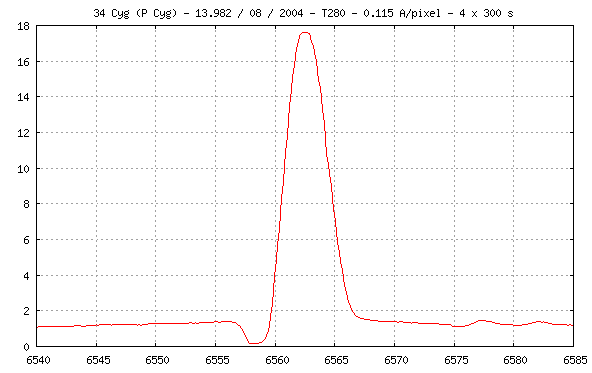
\includegraphics[scale=.40]{figures/34cygni.png}
\caption{The normalised spectrum of 34 Cygni around H$\alpha$.}
\end{figure}

It is hypothesised that distinct physical processes within these stars generate the respective line profiles \cite{hou2016catalog}. Beals was the first to demonstrate that P Cygni and Inverse P Cygni line profiles can be explained by the interaction between the stellar disk of a hot, massive young star and the expanding or contracting shell of gas surrounding the star \cite{1953PDAO....9....1B}. 

\begin{figure}[h]
\centering
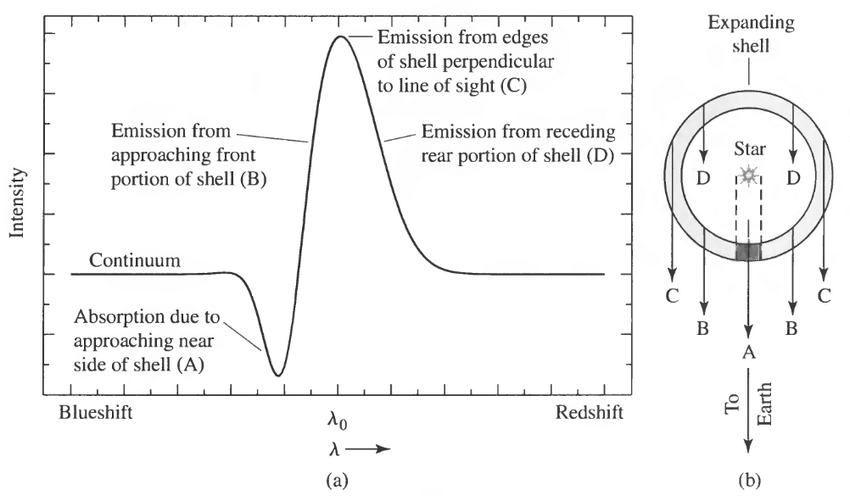
\includegraphics[scale=.40]{figures/expandingpcygni.png}
\caption{Cartoon depicting the physical mechanism by which a P Cygni line profile is generated. Reproduced from Kasai (2013)\cite{kasai2013type}.}
\end{figure}

The P Cygni line profile observed is thus a result of an expanding shell of gas around the main disk of the young hot star. The segment of this shell along the ling of sight contributes to the generation of the absorption line in the spectrum. An average or normal main sequence star will only show a significantly deep absorption line/trough near H$\alpha$. However, note that in the case of P Cygni, the regions B, C and D of the shell contribute to an emission line. This emission line can occur near H$\alpha$. As we move from B to C, the intensity of the emission line increases until we reach the edge of the shell. Beyond this point the shell is receding with respect to the line of sight and the intensity of the emission line decreases. It is believed that the opposite process occurs in the case of an inverse P Cygni star. In this case, the shell of gas is contracting and this inflow is responsible for the blue shifted emission line, often to the left of H$\alpha$.

\begin{figure}[h]
\centering
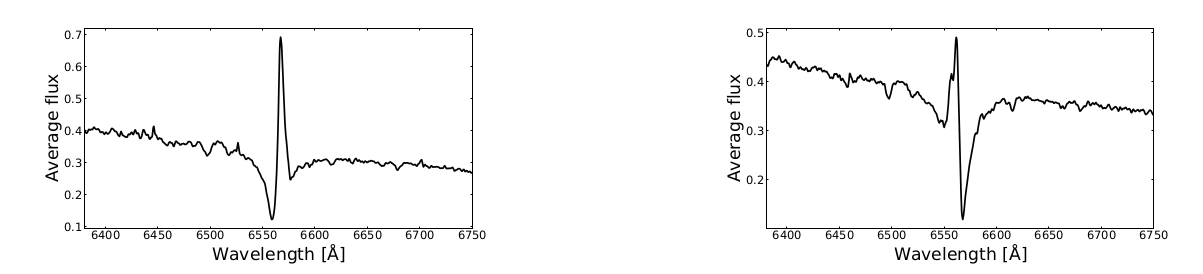
\includegraphics[scale=.50]{figures/p cygni and inverse p cygni.png}
\caption{A P Cygni spectrum (left) and an inverse P Cygni spectrum (right) from LAMOST Data Release 7. Reproduced from Zhang (2021)\cite{zhang2021catalog}.}
\end{figure}

\section{Morphological Classification}

One of the first modern attempts at identifying and characterising P Cygni stars was by Beals (1953) \cite{1953PDAO....9....1B}. This work compiled Northern Hemisphere observations of P Cygni stars into a comprehensive catalog. This catalog was compiled by examining spectra using the naked eye, during a period of observation between the years 1928 and 1946. The catalog was then used to generate hypotheses of how P Cygni stars may exchange material with their surroundings via accretions, inflows and outflows. The morphological properties of the spectra were then used to calculate the wind velocities of inflows and outflows. 

\begin{figure}[t]
\centering
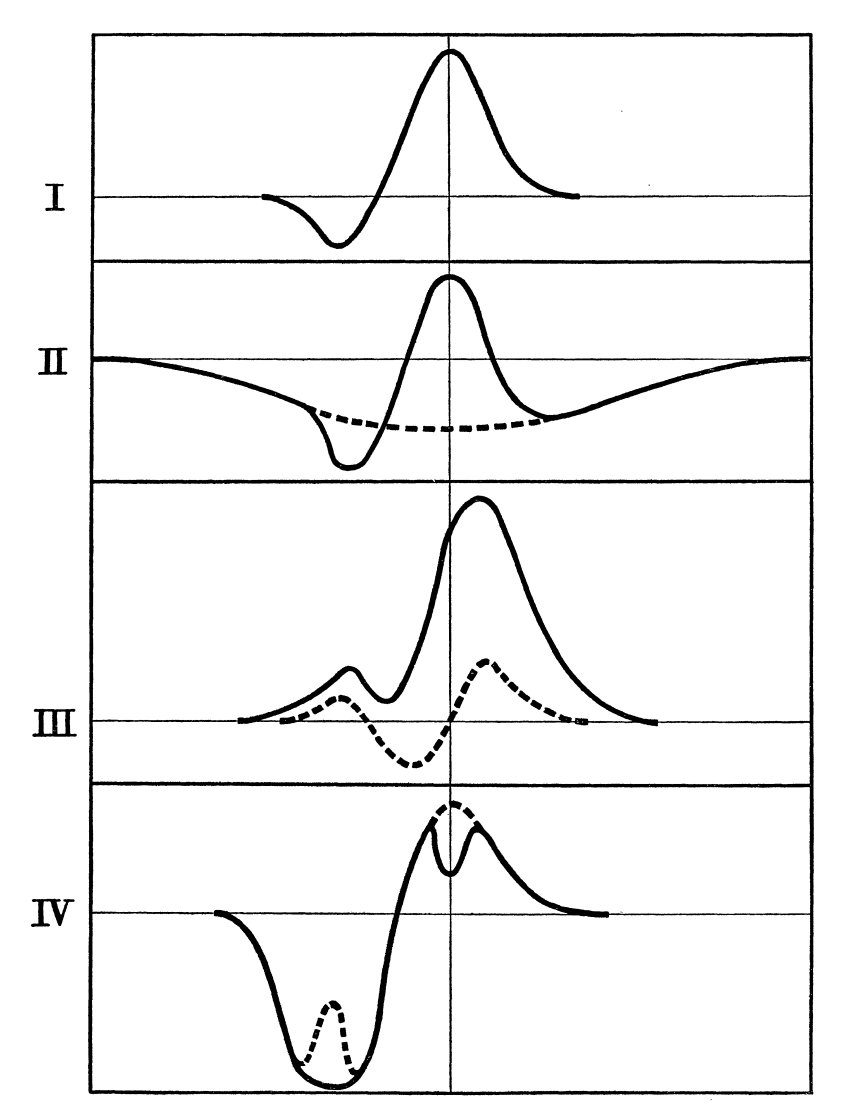
\includegraphics[scale=.30]{figures/beals class 1.png}
\caption{Primary P Cygni classes - the morphological classification of P Cygni spectra proposed by Beals (1953) \cite{1953PDAO....9....1B}.}
\end{figure}

The work also presents an early attempt at classification of P Cygni stars based on their morphologies. The classification provided by Beals is broader than modern schemes \cite{reipurth1996halpha}. In addition to the primary classes, Beals proposed a set of non-typical classes which were also considered to be P Cygni spectra. This work does not consider these non-typical classes to be P Cygni spectra but rather consider them to be a subgroup of emission line spectra. This approach is congruent with modern research \cite{vcotar2021galah}\cite{zhang2021catalog}\cite{reipurth1996halpha} which promote constraints on the classification of P Cygni and inverse P Cygni morphologies. 

Classification regimes since the 1950s have largely been manual i.e. visual inspection of spectra. However, over the last five to seven years semi-automated and automated methods have been explored by many groups. A more detailed discussion of these attempts are provided in Chapter 3.

\begin{figure}[h]
\centering
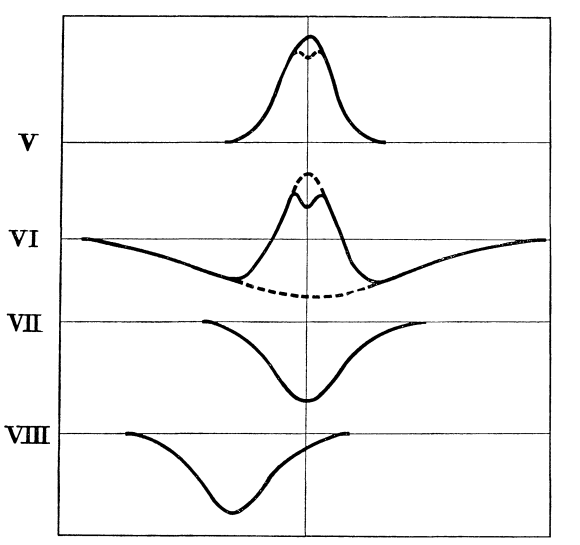
\includegraphics[scale=.50]{figures/beals class 2.png}
\caption{Non-typical P Cygni classes proposed by Beals.}
\end{figure}

\section{Importance}
The identification, classification and modelling of peculiar stars such as P Cygni and inverse P Cygni can provide significant insight into our understanding of stellar evolution and the physical processes that drive them. With the advent of modern large scale spectroscopic survey science, the importance of detecting these stars and modelling them using data driven methods has gained prominence.

Modern spectroscopic surveys generate data from millions of sources. These "million star surveys" generate a significant volume of data. Thus, it has become impractical to study these sources using manual methods. In order to generate stellar parameters from survey spectra, modern researchers rely on generalised automated pipelines. These generalised pipelines rely on templates and models that assume a non-peculiar baseline. 

It has been demonstrated that such an approach has an impact on the accurate determination of effective temperature \cite{cayrel2011halpha}\cite{amarsi2018effective}\cite{giribaldi2019accurate}. The effect on computing stellar masses has also been well documented \cite{ness2016spectroscopic}\cite{bergemann2016gaia}. Thus the identification and characterisation of peculiar stars such as P Cygni and inverse P Cygni stars has a direct impact on the accuracy of automated estimation of stellar parameters in large scale spectroscopic surveys. 

\begin{table}[]
\begin{center}
\begin{tabular}{|c|c|c|}
\hline
\textbf{Survey} & \textbf{Number of Spectra} & \textbf{Resolution} \\ \hline
Gaia ESO        & $\sim$150,000              & High                \\ \hline
LAMOST          & $\sim$10,000,000           & Low                 \\ \hline
APOGEE          & $\sim$250,000              & High                \\ \hline
RAVE            & $\sim$600,000              & High                \\ \hline
GAIA            & $\sim$100,000,000          & Low                 \\ \hline
\end{tabular}
\caption{Modern spectroscopic surveys generate high volume, and often high resolution data that are analysed by automated pipelines.}
\label{table:draglift1}
\end{center}
\end{table}

\section{The GALAH Survey}

The GALAH survey is a million star Milky Way spectroscopic survey which uses the HERMES spectrograph at the Anglo Australian Telescope \cite{de2015galah} \cite{buder2021galah+}. The GALAH survey is currently in its third data release (DR3) and contains more than 600,000 spectra. The volume of data being generated by the GALAH survey has necessitated the use of semi-automated and automated data analytics pipelines over manual methods.

\section{Goals}

REWRITE THIS

This thesis will use a novel data driven approach to cluster, classify and identify PCT stars in GALAH DR3. Once these PCT stars have been identified, the thesis will characterise these stars with reference to stellar parameters. This thesis will model the spectra using optimisation techniques and gaussian mixture models (GMM) to estimate the stellar wind velocity directly from the normalised spectra of the PCT stars (Zhang et al. 2021; Traven et al. 2015).

The focus of this literature review is twofold. One aspect of the review will be on the scientific work done on P-Cygni stars in particular and emission stars in general, and their relevance to the thesis. The second aspect will be a brief survey of recent computational methods that are relevant to the thesis, with a special focus on machine learning and signal processing methods. 



